\documentclass{beamer}
\usetheme{Antibes}
\usepackage{microtype}
\usepackage{graphicx}
\title{The Role of Bartle’s Gamer Types in Gamified Higher Education}
\author{William Seymour}
\institute{University of Warwick}
\date{March 12th, 2015}
\beamertemplatenavigationsymbolsempty

\begin{document}
	\begin{frame}
		\titlepage
	\end{frame}
	\frame{
		\frametitle{Presentation Overview}
		\begin{enumerate}
			\item What is gamification?
			\item What are Bartle's gamer types?
			\item Research undertaken
			\item Conclusion and further work
			\item Project evaluation
		\end{enumerate}
	}
	
	\frame{
		\frametitle{Gamification}
		\begin{quotation}
			``The use of game design elements \\ in non-game contexts''\footnote{Definition from “From game design elements to gamefulness by Detarding et al. (2011)}
		\end{quotation}
		
		Or, put another way, transplanting the game mechanics that make games engaging into other media with the aim of driving engagement.
		\newline
		
		It is important to make the distinction between \textit{games} and \textit{gamified activities}.
	}
	
	\frame{
		\frametitle{Gamification}
		Though it existed before, the term really spiked in usage from \textasciitilde2010\footnote{Google Trends image: proportion of gamification searches relative to the peak}. Gamification has psychological roots in operant conditioning (cf. B. F. Skinner) and Self Determination Theory.
		
			\begin{figure}
				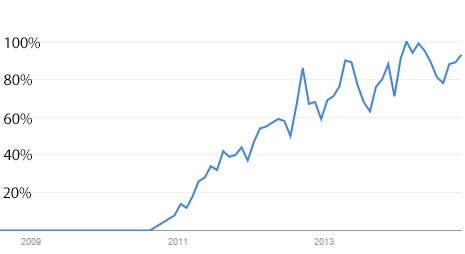
\includegraphics[width=0.5\linewidth]{../img/usage-graph.png}
			\end{figure}
			
			Usage of time over skill as a method of determining worth makes all players feel involved instead of just the top few.
	}
	
	\frame{
		\frametitle{Learning Analytics}
		The concept of using data analysis to inform the education process, giving a more personalised experience for students. Makes it possible to match students together by ability or learning style.
		
		\begin{figure}
			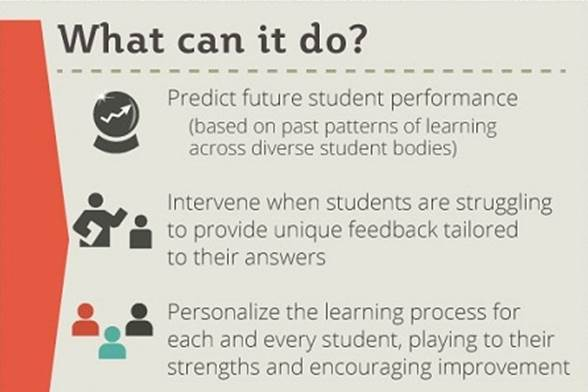
\includegraphics[width=0.6\linewidth]{../img/infographic.jpg}
			\footnote{Image part of an infographic by www.opencolleges.edu.au}
		\end{figure}
	}
	
\end{document}